\chapter{Metodi HTTP}

\begin{tcolorbox}[title=Mappa del capitolo]
Metodi HTTP principali, GET, POST, PUT, PATCH, DELETE, OPTIONS, HEAD, Idempotenza, Safety, Request/Response completi, Esempi pratici, Diagrammi flow, When to use, Best practices, Errori comuni.
\end{tcolorbox}

\section*{Obiettivi di apprendimento}
\begin{itemize}
  \item Comprendere semantica di ogni metodo HTTP
  \item Applicare correttamente GET, POST, PUT, PATCH, DELETE
  \item Distinguere tra safe e unsafe methods
  \item Comprendere idempotenza e sue implicazioni
  \item Scegliere metodo appropriato per ogni operazione
  \item Evitare errori comuni (GET per modifiche, POST per tutto)
\end{itemize}

\section{Panoramica Metodi HTTP}

I metodi HTTP (o \textbf{verbs}) definiscono l'\textbf{azione} da eseguire su una risorsa. RFC 7231 definisce 9 metodi, di cui 5 fondamentali per REST:

\begin{table}[h]
\centering
\begin{tabular}{|l|l|c|c|p{4cm}|}
\hline
\textbf{Metodo} & \textbf{Operazione} & \textbf{Safe} & \textbf{Idempotent} & \textbf{Uso REST} \\ \hline
GET & Leggi & Sì & Sì & Recupera risorsa \\ \hline
POST & Crea & No & No & Crea nuova risorsa \\ \hline
PUT & Sostituisci & No & Sì & Aggiorna/sostituisce \\ \hline
PATCH & Modifica & No & No* & Modifica parziale \\ \hline
DELETE & Elimina & No & Sì & Rimuovi risorsa \\ \hline
HEAD & Metadata & Sì & Sì & Come GET senza body \\ \hline
OPTIONS & Capacità & Sì & Sì & Descrive opzioni \\ \hline
\end{tabular}
\caption{Metodi HTTP principali}
\end{table}

\textit{* PATCH può essere idempotente se implementato correttamente}

\section{Proprietà dei Metodi}

\subsection{Safe Methods}

Un metodo è \textbf{safe} se non modifica lo stato del server. Operazioni di sola lettura.

\textbf{Safe methods}: GET, HEAD, OPTIONS, TRACE

\begin{tcolorbox}[colback=blue!5, colframe=blue!60, title=Definizione Safe]
Un metodo è safe se la sua semantica è \textbf{essenzialmente read-only}. Il client non richiede né si aspetta modifiche di stato sul server.
\end{tcolorbox}

\textbf{Implicazioni}:
\begin{itemize}
    \item Crawler e bot possono chiamare safe methods senza preoccupazioni
    \item Prefetching e caching sicuri
    \item Nessun side effect atteso
\end{itemize}

\textbf{Nota}: "Safe" è semantico, non garantisce che server non cambi (es: logging, analytics).

\subsection{Idempotenza}

Un metodo è \textbf{idempotente} se \textbf{N richieste identiche} hanno lo \textbf{stesso effetto} di una singola richiesta.

\textbf{Idempotent methods}: GET, PUT, DELETE, HEAD, OPTIONS

\begin{tcolorbox}[colback=green!5, colframe=green!60, title=Definizione Idempotenza]
Formalmente: $f(f(x)) = f(x)$

Applicando operazione idempotente multiple volte, lo stato finale è uguale ad applicarla una volta.
\end{tcolorbox}

\textbf{Esempio idempotenza}:
\begin{lstlisting}[caption=PUT è idempotente]
# Prima richiesta
PUT /api/users/123 HTTP/1.1
Content-Type: application/json

{"name": "Mario Rossi", "email": "mario@example.com"}

# HTTP/1.1 200 OK
# User 123 ora ha name="Mario Rossi"

# Seconda richiesta identica
PUT /api/users/123 HTTP/1.1
Content-Type: application/json

{"name": "Mario Rossi", "email": "mario@example.com"}

# HTTP/1.1 200 OK
# User 123 ha ANCORA name="Mario Rossi" (stesso stato)
\end{lstlisting}

\textbf{Esempio NON idempotente}:
\begin{lstlisting}[caption=POST NON è idempotente]
# Prima richiesta
POST /api/users HTTP/1.1
Content-Type: application/json

{"name": "Mario Rossi"}

# HTTP/1.1 201 Created
# Location: /api/users/123
# Creato user con ID 123

# Seconda richiesta identica
POST /api/users HTTP/1.1
Content-Type: application/json

{"name": "Mario Rossi"}

# HTTP/1.1 201 Created
# Location: /api/users/124
# Creato ALTRO user con ID 124 (stato diverso!)
\end{lstlisting}

\textbf{Perché idempotenza è importante}:
\begin{itemize}
    \item \textbf{Retry safety}: Se richiesta fallisce per network error, client può ritentare
    \item \textbf{Distributed systems}: Garantisce consistency in caso di duplicazione messaggi
    \item \textbf{Predictability}: Comportamento prevedibile per client
\end{itemize}

\section{GET - Read}

\subsection{Semantica GET}

\textbf{Scopo}: Recuperare rappresentazione di una risorsa.

\textbf{Caratteristiche}:
\begin{itemize}
    \item Safe: sola lettura
    \item Idempotent: multiple GET → stesso risultato
    \item Cacheable: response può essere cached
    \item NO request body (parametri in query string)
\end{itemize}

\subsection{Esempio GET - Singola Risorsa}

\begin{lstlisting}[caption=GET singolo user]
GET /api/v1/users/123 HTTP/1.1
Host: api.example.com
Accept: application/json
Authorization: Bearer eyJhbGc...

HTTP/1.1 200 OK
Content-Type: application/json
Cache-Control: max-age=300
ETag: "abc123"

{
  "id": 123,
  "name": "Mario Rossi",
  "email": "mario.rossi@example.com",
  "role": "admin",
  "created_at": "2025-01-15T10:30:00Z"
}
\end{lstlisting}

\subsection{Esempio GET - Collection}

\begin{lstlisting}[caption=GET lista users con filtering]
GET /api/v1/users?role=admin&status=active&page=1&limit=10 HTTP/1.1
Host: api.example.com
Accept: application/json

HTTP/1.1 200 OK
Content-Type: application/json
X-Total-Count: 42
Link: </api/v1/users?page=2&limit=10>; rel="next"

{
  "data": [
    {
      "id": 123,
      "name": "Mario Rossi",
      "email": "mario@example.com"
    },
    {
      "id": 124,
      "name": "Luigi Verdi",
      "email": "luigi@example.com"
    }
  ],
  "pagination": {
    "page": 1,
    "limit": 10,
    "total": 42,
    "pages": 5
  }
}
\end{lstlisting}

\subsection{GET con Conditional Request}

\begin{lstlisting}[caption=GET con ETag per evitare transfer non necessari]
# Prima richiesta
GET /api/v1/users/123 HTTP/1.1

HTTP/1.1 200 OK
ETag: "33a64df551425fcc"
Content-Type: application/json

{"id": 123, "name": "Mario"}

# Seconda richiesta con If-None-Match
GET /api/v1/users/123 HTTP/1.1
If-None-Match: "33a64df551425fcc"

HTTP/1.1 304 Not Modified
# Nessun body, client usa cache locale
\end{lstlisting}

\subsection{Quando usare GET}

\textbf{Usare GET per}:
\begin{itemize}
    \item Recuperare singola risorsa: \texttt{GET /users/123}
    \item Recuperare collection: \texttt{GET /users}
    \item Search/filtering: \texttt{GET /products?category=electronics}
    \item Operazioni read-only
\end{itemize}

\textbf{NON usare GET per}:
\begin{itemize}
    \item Modificare stato server (usare POST/PUT/PATCH/DELETE)
    \item Operazioni sensibili in URL (password, token visibili in logs)
    \item Request body (usare POST se dati complessi)
\end{itemize}

\begin{tcolorbox}[colback=red!5, colframe=red!60, title=Errore comune]
\textbf{MAI fare}:
\begin{lstlisting}
GET /api/users/123/delete  # NO! Violazione safe property
GET /api/users/create?name=Mario  # NO! GET non crea risorse
\end{lstlisting}

Crawler e proxy possono pre-fetch GET, causando eliminazioni/creazioni accidentali!
\end{tcolorbox}

\section{POST - Create}

\subsection{Semantica POST}

\textbf{Scopo}: Creare nuova risorsa o eseguire operazione complessa.

\textbf{Caratteristiche}:
\begin{itemize}
    \item NOT safe: modifica stato
    \item NOT idempotent: multiple POST → risorse multiple
    \item Request body obbligatorio (payload)
    \item Server assegna ID alla nuova risorsa
\end{itemize}

\subsection{Esempio POST - Creazione Risorsa}

\begin{lstlisting}[caption=POST crea nuovo user]
POST /api/v1/users HTTP/1.1
Host: api.example.com
Content-Type: application/json
Authorization: Bearer eyJhbGc...

{
  "name": "Mario Rossi",
  "email": "mario.rossi@example.com",
  "role": "user"
}

HTTP/1.1 201 Created
Location: /api/v1/users/125
Content-Type: application/json

{
  "id": 125,
  "name": "Mario Rossi",
  "email": "mario.rossi@example.com",
  "role": "user",
  "created_at": "2025-11-15T14:22:00Z"
}
\end{lstlisting}

\textbf{Elementi chiave}:
\begin{itemize}
    \item Status: \textbf{201 Created}
    \item Header \textbf{Location}: URI della risorsa creata
    \item Response body: rappresentazione completa risorsa creata
\end{itemize}

\subsection{POST per Operazioni Complesse}

POST può essere usato per operazioni non mappabili a CRUD:

\begin{lstlisting}[caption=POST per operazione custom (search complessa)]
POST /api/v1/users/search HTTP/1.1
Content-Type: application/json

{
  "filters": {
    "age": {"min": 18, "max": 65},
    "roles": ["admin", "moderator"],
    "location": {
      "country": "IT",
      "city": "Milano"
    }
  },
  "sort": [
    {"field": "created_at", "order": "desc"}
  ],
  "pagination": {
    "page": 1,
    "limit": 20
  }
}

HTTP/1.1 200 OK
Content-Type: application/json

{
  "results": [...],
  "total": 152
}
\end{lstlisting}

\textbf{Nota}: Query complessa in POST body permette strutture che non stanno in query string.

\subsection{POST per Sub-risorse}

\begin{lstlisting}[caption=POST crea comment su post]
POST /api/v1/posts/456/comments HTTP/1.1
Content-Type: application/json

{
  "author": "Mario",
  "text": "Great article!"
}

HTTP/1.1 201 Created
Location: /api/v1/posts/456/comments/789
Content-Type: application/json

{
  "id": 789,
  "post_id": 456,
  "author": "Mario",
  "text": "Great article!",
  "created_at": "2025-11-15T14:25:00Z"
}
\end{lstlisting}

\subsection{Quando usare POST}

\textbf{Usare POST per}:
\begin{itemize}
    \item Creare nuova risorsa: \texttt{POST /users}
    \item Creare sub-risorsa: \texttt{POST /users/123/orders}
    \item Operazioni complesse: \texttt{POST /users/search}
    \item Triggering actions: \texttt{POST /orders/123/cancel}
    \item File upload
\end{itemize}

\section{PUT - Update/Replace}

\subsection{Semantica PUT}

\textbf{Scopo}: Sostituire interamente una risorsa esistente.

\textbf{Caratteristiche}:
\begin{itemize}
    \item NOT safe: modifica stato
    \item Idempotent: PUT ripetuto → stesso stato
    \item Request body contiene rappresentazione completa
    \item Client specifica URI della risorsa
\end{itemize}

\subsection{PUT vs POST}

\textbf{Differenza chiave}: Chi decide l'URI?

\begin{itemize}
    \item \textbf{POST}: Server decide URI (assegna ID)
    \item \textbf{PUT}: Client specifica URI completo
\end{itemize}

\subsection{Esempio PUT - Replace completo}

\begin{lstlisting}[caption=PUT sostituisce user completamente]
PUT /api/v1/users/123 HTTP/1.1
Content-Type: application/json
Authorization: Bearer eyJhbGc...

{
  "name": "Mario Rossi Updated",
  "email": "mario.updated@example.com",
  "role": "admin",
  "phone": "+39 123 456 7890"
}

HTTP/1.1 200 OK
Content-Type: application/json

{
  "id": 123,
  "name": "Mario Rossi Updated",
  "email": "mario.updated@example.com",
  "role": "admin",
  "phone": "+39 123 456 7890",
  "updated_at": "2025-11-15T14:30:00Z"
}
\end{lstlisting}

\textbf{Importante}: PUT sostituisce \textbf{intera} risorsa. Campi omessi vengono rimossi/resettati.

\subsection{PUT Idempotente - Esempio}

\begin{lstlisting}[caption=PUT ripetuto ha stesso effetto]
# Prima richiesta
PUT /api/v1/users/123 HTTP/1.1
Content-Type: application/json

{"name": "Mario", "email": "mario@example.com"}

# User 123: name=Mario, email=mario@example.com

# Seconda richiesta IDENTICA (network retry)
PUT /api/v1/users/123 HTTP/1.1
Content-Type: application/json

{"name": "Mario", "email": "mario@example.com"}

# User 123: ANCORA name=Mario, email=mario@example.com
# Stato identico, nessuna duplicazione
\end{lstlisting}

\subsection{PUT per Upsert}

PUT può creare risorsa se non esiste (upsert pattern):

\begin{lstlisting}[caption=PUT upsert - crea se non esiste]
PUT /api/v1/users/999 HTTP/1.1
Content-Type: application/json

{"name": "Nuovo User", "email": "nuovo@example.com"}

# Se user 999 non esiste
HTTP/1.1 201 Created
Location: /api/v1/users/999

# Se user 999 già esiste
HTTP/1.1 200 OK
\end{lstlisting}

\textbf{Nota}: Pattern upsert non sempre consigliato (preferire POST per create, PUT per update).

\section{PATCH - Partial Update}

\subsection{Semantica PATCH}

\textbf{Scopo}: Modificare \textbf{parzialmente} una risorsa esistente.

\textbf{Caratteristiche}:
\begin{itemize}
    \item NOT safe: modifica stato
    \item Può essere idempotent (dipende da implementazione)
    \item Request body: solo campi da modificare
    \item Standard: JSON Patch (RFC 6902) o JSON Merge Patch (RFC 7396)
\end{itemize}

\subsection{PATCH vs PUT}

\begin{itemize}
    \item \textbf{PUT}: Sostituisce intera risorsa (campi omessi → rimossi)
    \item \textbf{PATCH}: Modifica solo campi specificati (altri invariati)
\end{itemize}

\subsection{Esempio PATCH - Simple Merge}

\begin{lstlisting}[caption=PATCH modifica solo email]
PATCH /api/v1/users/123 HTTP/1.1
Content-Type: application/json

{
  "email": "mario.new@example.com"
}

HTTP/1.1 200 OK
Content-Type: application/json

{
  "id": 123,
  "name": "Mario Rossi",  // Invariato
  "email": "mario.new@example.com",  // Modificato
  "role": "admin",  // Invariato
  "updated_at": "2025-11-15T14:35:00Z"
}
\end{lstlisting}

\subsection{JSON Patch (RFC 6902)}

Formato standardizzato per patch complesse:

\begin{lstlisting}[caption=PATCH con JSON Patch RFC 6902]
PATCH /api/v1/users/123 HTTP/1.1
Content-Type: application/json-patch+json

[
  { "op": "replace", "path": "/email", "value": "new@example.com" },
  { "op": "add", "path": "/phone", "value": "+39 123 456" },
  { "op": "remove", "path": "/temporary_field" }
]

HTTP/1.1 200 OK
\end{lstlisting}

\textbf{Operazioni JSON Patch}:
\begin{itemize}
    \item \texttt{add}: Aggiungi campo
    \item \texttt{remove}: Rimuovi campo
    \item \texttt{replace}: Sostituisci valore
    \item \texttt{move}: Sposta valore
    \item \texttt{copy}: Copia valore
    \item \texttt{test}: Verifica valore (condizionale)
\end{itemize}

\subsection{Quando usare PATCH}

\textbf{Usare PATCH per}:
\begin{itemize}
    \item Modificare pochi campi di risorsa grande
    \item Bandwidth optimization (mobile)
    \item Partial updates atomiche
\end{itemize}

\textbf{Usare PUT invece}:
\begin{itemize}
    \item Update completo più semplice da implementare
    \item Tutti i campi sempre inviati (form completo)
\end{itemize}

\section{DELETE - Remove}

\subsection{Semantica DELETE}

\textbf{Scopo}: Eliminare una risorsa.

\textbf{Caratteristiche}:
\begin{itemize}
    \item NOT safe: modifica stato
    \item Idempotent: DELETE ripetuto → stesso stato (risorsa assente)
    \item NO request body (solitamente)
    \item Response può essere empty (204) o con dettagli (200)
\end{itemize}

\subsection{Esempio DELETE - Success}

\begin{lstlisting}[caption=DELETE risorsa con successo]
DELETE /api/v1/users/123 HTTP/1.1
Authorization: Bearer eyJhbGc...

HTTP/1.1 204 No Content
# Nessun body, risorsa eliminata
\end{lstlisting}

\textbf{Alternative response}:
\begin{lstlisting}[caption=DELETE con response body]
DELETE /api/v1/users/123 HTTP/1.1

HTTP/1.1 200 OK
Content-Type: application/json

{
  "message": "User deleted successfully",
  "deleted_id": 123,
  "deleted_at": "2025-11-15T14:40:00Z"
}
\end{lstlisting}

\subsection{DELETE Idempotente}

\begin{lstlisting}[caption=DELETE ripetuto è idempotente]
# Prima richiesta
DELETE /api/v1/users/123 HTTP/1.1

HTTP/1.1 204 No Content
# Risorsa eliminata

# Seconda richiesta (retry)
DELETE /api/v1/users/123 HTTP/1.1

# Opzione 1: Considerare successo (idempotenza)
HTTP/1.1 204 No Content

# Opzione 2: Indicare risorsa già assente
HTTP/1.1 404 Not Found
{
  "error": "User not found"
}
\end{lstlisting}

\textbf{Debate}: 204 o 404 per DELETE su risorsa già assente?

\begin{itemize}
    \item \textbf{204 (idempotente)}: Stato finale identico (risorsa assente)
    \item \textbf{404 (preciso)}: Risorsa non esiste, impossibile eliminarla
\end{itemize}

Best practice: \textbf{204} per mantenere idempotenza.

\subsection{Soft Delete vs Hard Delete}

\textbf{Hard Delete}: Risorsa fisicamente rimossa da database
\begin{lstlisting}[caption=Hard delete - risorsa rimossa permanentemente]
DELETE /api/v1/users/123 HTTP/1.1

HTTP/1.1 204 No Content
# User completamente rimosso dal database
\end{lstlisting}

\textbf{Soft Delete}: Risorsa marcata come deleted (flag)
\begin{lstlisting}[caption=Soft delete - risorsa marcata come eliminata]
DELETE /api/v1/users/123 HTTP/1.1

HTTP/1.1 200 OK
Content-Type: application/json

{
  "id": 123,
  "name": "Mario",
  "deleted": true,
  "deleted_at": "2025-11-15T14:45:00Z"
}

# GET successivo
GET /api/v1/users/123 HTTP/1.1

HTTP/1.1 410 Gone
# Risorsa esiste ma è stata eliminata (soft delete)
\end{lstlisting}

\section{HEAD - Metadata Only}

\textbf{Scopo}: Come GET ma solo headers, senza body.

\textbf{Uso}:
\begin{itemize}
    \item Verificare esistenza risorsa
    \item Controllare dimensione (Content-Length)
    \item Validare cache (ETag, Last-Modified)
\end{itemize}

\begin{lstlisting}[caption=HEAD per verificare risorsa]
HEAD /api/v1/users/123 HTTP/1.1

HTTP/1.1 200 OK
Content-Type: application/json
Content-Length: 245
ETag: "abc123"
Last-Modified: Wed, 15 Nov 2025 10:00:00 GMT
# Nessun body
\end{lstlisting}

\section{OPTIONS - Capabilities}

\textbf{Scopo}: Descrivere metodi HTTP supportati dalla risorsa.

\textbf{Uso principale}: CORS preflight requests

\begin{lstlisting}[caption=OPTIONS per CORS]
OPTIONS /api/v1/users/123 HTTP/1.1
Origin: https://example.com
Access-Control-Request-Method: DELETE

HTTP/1.1 204 No Content
Allow: GET, PUT, PATCH, DELETE, OPTIONS
Access-Control-Allow-Origin: https://example.com
Access-Control-Allow-Methods: GET, PUT, PATCH, DELETE
Access-Control-Max-Age: 86400
\end{lstlisting}

\section{Diagramma HTTP Request/Response Flow}

\begin{figure}[h]
\centering
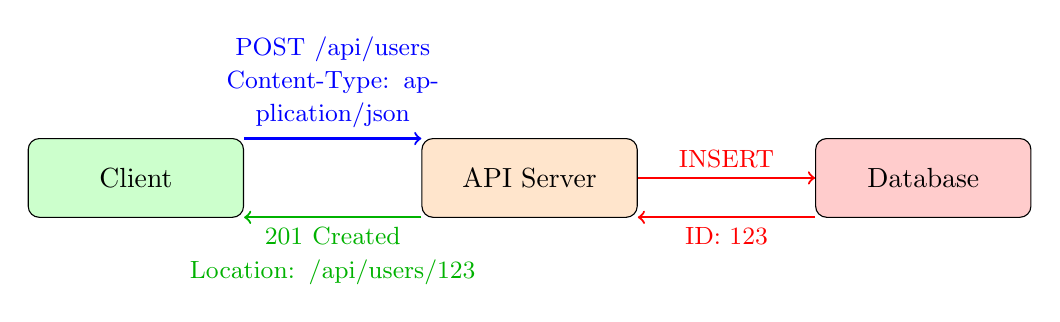
\begin{tikzpicture}[
    node distance=2.5cm,
    box/.style={rectangle, draw, fill=blue!20, text width=2.5cm, text centered, minimum height=1cm, rounded corners},
    arrow/.style={->, thick}
]
    % Client
    \node[box, fill=green!20] (client) {Client};

    % API Server
    \node[box, fill=orange!20, right of=client, node distance=5cm] (server) {API Server};

    % Database
    \node[box, fill=red!20, right of=server, node distance=5cm] (db) {Database};

    % Request
    \draw[arrow, blue] (client.20) -- node[above, text width=4cm, align=center] {\small POST /api/users\\Content-Type: application/json} (server.160);

    % Server → DB
    \draw[arrow, red] (server.0) -- node[above] {\small INSERT} (db.180);

    % DB → Server
    \draw[arrow, red] (db.200) -- node[below] {\small ID: 123} (server.340);

    % Response
    \draw[arrow, green!70!black] (server.200) -- node[below, text width=4cm, align=center] {\small 201 Created\\Location: /api/users/123} (client.340);

\end{tikzpicture}
\caption{HTTP Flow: POST create user}
\end{figure}

\section{Best Practices}

\begin{tcolorbox}[title=Best Practices HTTP Methods]
\begin{enumerate}
    \item \textbf{GET per read-only}: Mai modificare stato con GET
    \item \textbf{POST per create}: Lascia server assegnare ID
    \item \textbf{PUT per replace}: Invia rappresentazione completa
    \item \textbf{PATCH per partial}: Modifica solo campi necessari
    \item \textbf{DELETE è idempotente}: 204 anche se già eliminato
    \item \textbf{Status codes corretti}: 201 per POST, 204 per DELETE
    \item \textbf{Location header}: Sempre in 201 Created
    \item \textbf{Safe methods cacheable}: Implementa ETag per GET
    \item \textbf{Idempotenza per retry}: PUT/DELETE sicuri da ritentare
    \item \textbf{Validation}: Valida input prima di processare
\end{enumerate}
\end{tcolorbox}

\begin{tcolorbox}[colback=red!5, colframe=red!60, title=Errori comuni]
\begin{itemize}
    \item \textbf{GET per delete}: \texttt{GET /users/123/delete} (PERICOLOSO!)
    \item \textbf{POST per tutto}: Ignora semantica altri metodi
    \item \textbf{PUT senza idempotenza}: Incrementi in PUT violano idempotenza
    \item \textbf{PATCH completo}: Se modifichi tutto, usa PUT
    \item \textbf{DELETE con body}: Semanticamente scorretto
    \item \textbf{Status codes sbagliati}: 200 OK per DELETE invece di 204
    \item \textbf{Mancanza Location}: POST 201 senza Location header
\end{itemize}
\end{tcolorbox}

\section{Riepilogo}

\begin{table}[h]
\centering
\small
\begin{tabular}{|l|l|l|l|l|}
\hline
\textbf{Metodo} & \textbf{CRUD} & \textbf{Safe} & \textbf{Idempotent} & \textbf{Status Success} \\ \hline
GET & Read & Sì & Sì & 200 OK \\ \hline
POST & Create & No & No & 201 Created \\ \hline
PUT & Update/Replace & No & Sì & 200 OK / 204 No Content \\ \hline
PATCH & Update Partial & No & No* & 200 OK \\ \hline
DELETE & Delete & No & Sì & 204 No Content / 200 OK \\ \hline
HEAD & Read metadata & Sì & Sì & 200 OK (no body) \\ \hline
OPTIONS & Metadata & Sì & Sì & 204 No Content \\ \hline
\end{tabular}
\caption{Riepilogo metodi HTTP}
\end{table}

\section*{Esercizi}

\begin{enumerate}
    \item Implementa endpoint CRUD completo per risorsa \texttt{/products}
    \item Progetta API per blog: POST create, PATCH update, DELETE
    \item Implementa idempotenza: gestisci retry duplicati con idempotency-key
    \item Test ETag caching: verifica 304 Not Modified
    \item Implementa JSON Patch RFC 6902 per update complessi
    \item Confronta bandwidth: PUT vs PATCH per update singolo campo
\end{enumerate}

\section*{Riferimenti}

\begin{itemize}
    \item RFC 7231 - HTTP/1.1 Semantics and Content: \url{https://tools.ietf.org/html/rfc7231}
    \item RFC 5789 - PATCH Method: \url{https://tools.ietf.org/html/rfc5789}
    \item RFC 6902 - JSON Patch: \url{https://tools.ietf.org/html/rfc6902}
    \item RFC 7396 - JSON Merge Patch: \url{https://tools.ietf.org/html/rfc7396}
\end{itemize}
